\pagestyle{fancy}
\onecolumn{}
\begin{figure}
\begin{adjustbox}{minipage=7.0in,frame}
% \begin{adjustbox}{width=7in,totalheight=7in,frame}
\vspace{2.5mm}
\centering

% \hspace{5mm}%
\begin{subfigure}[t]{.45\linewidth}
    \centering
    \captionsetup[subfigure]{}
    \caption{Gender.}\label{fig:shapsumgender}
    % 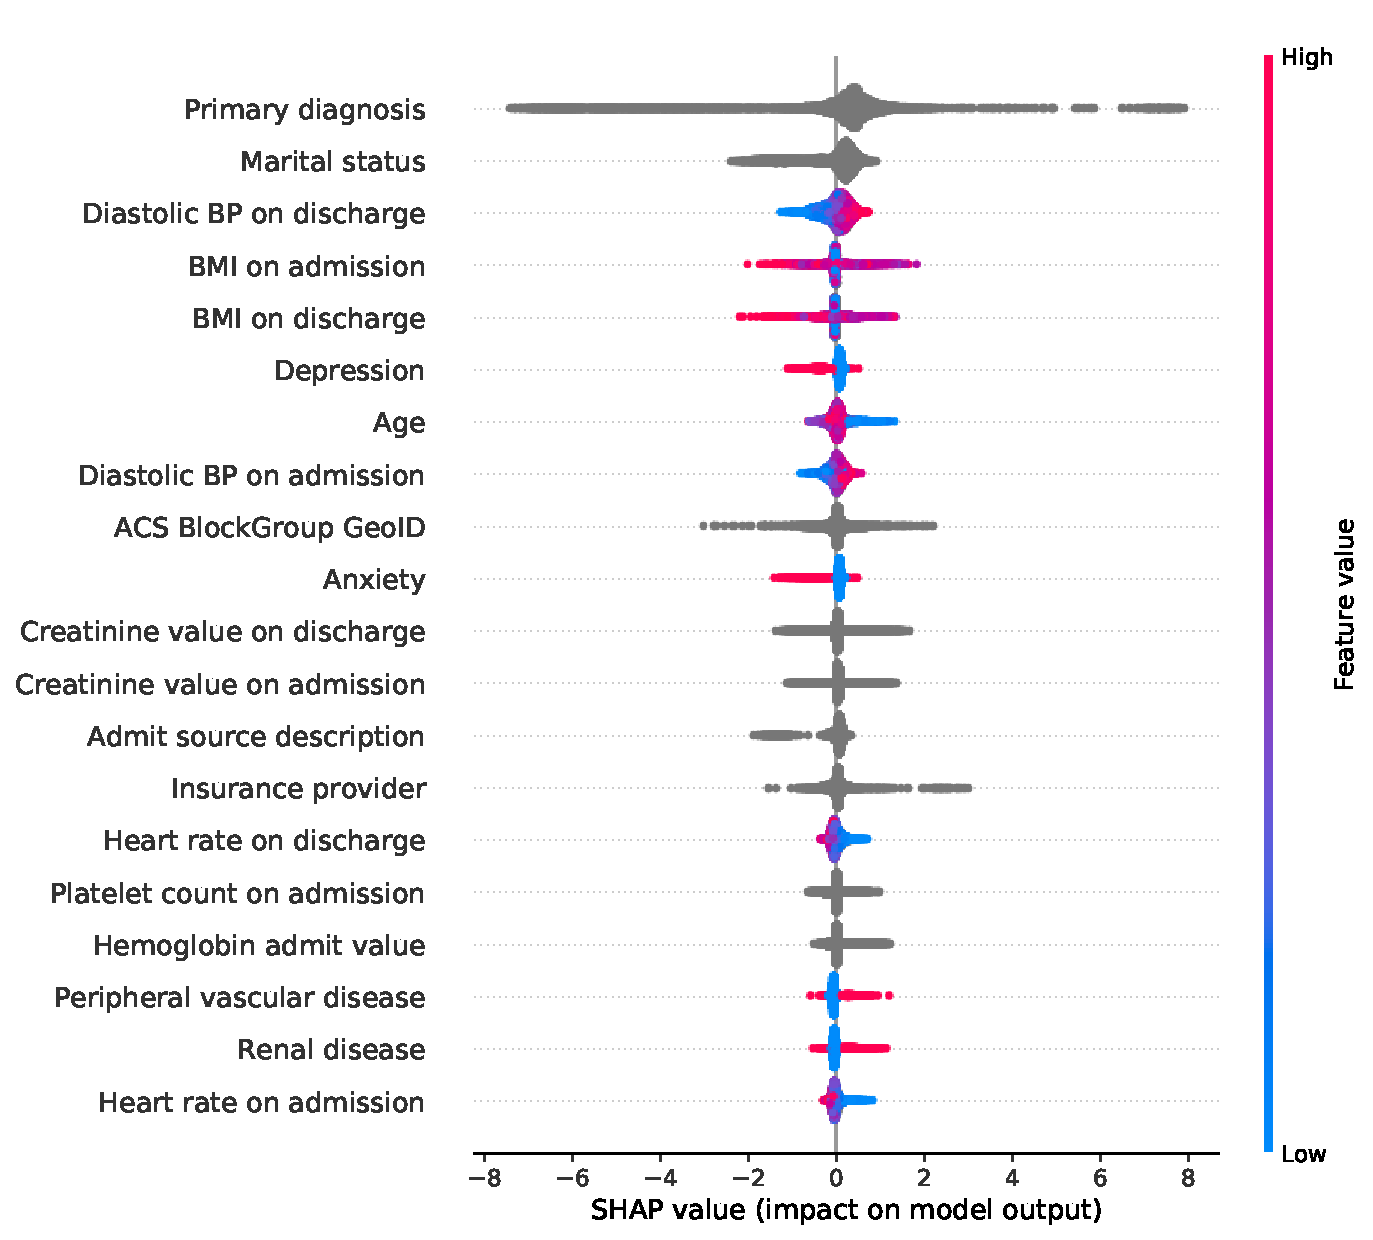
\includegraphics[width=\linewidth,keepaspectratio]{other/gender_SHAP_summary.pdf}
    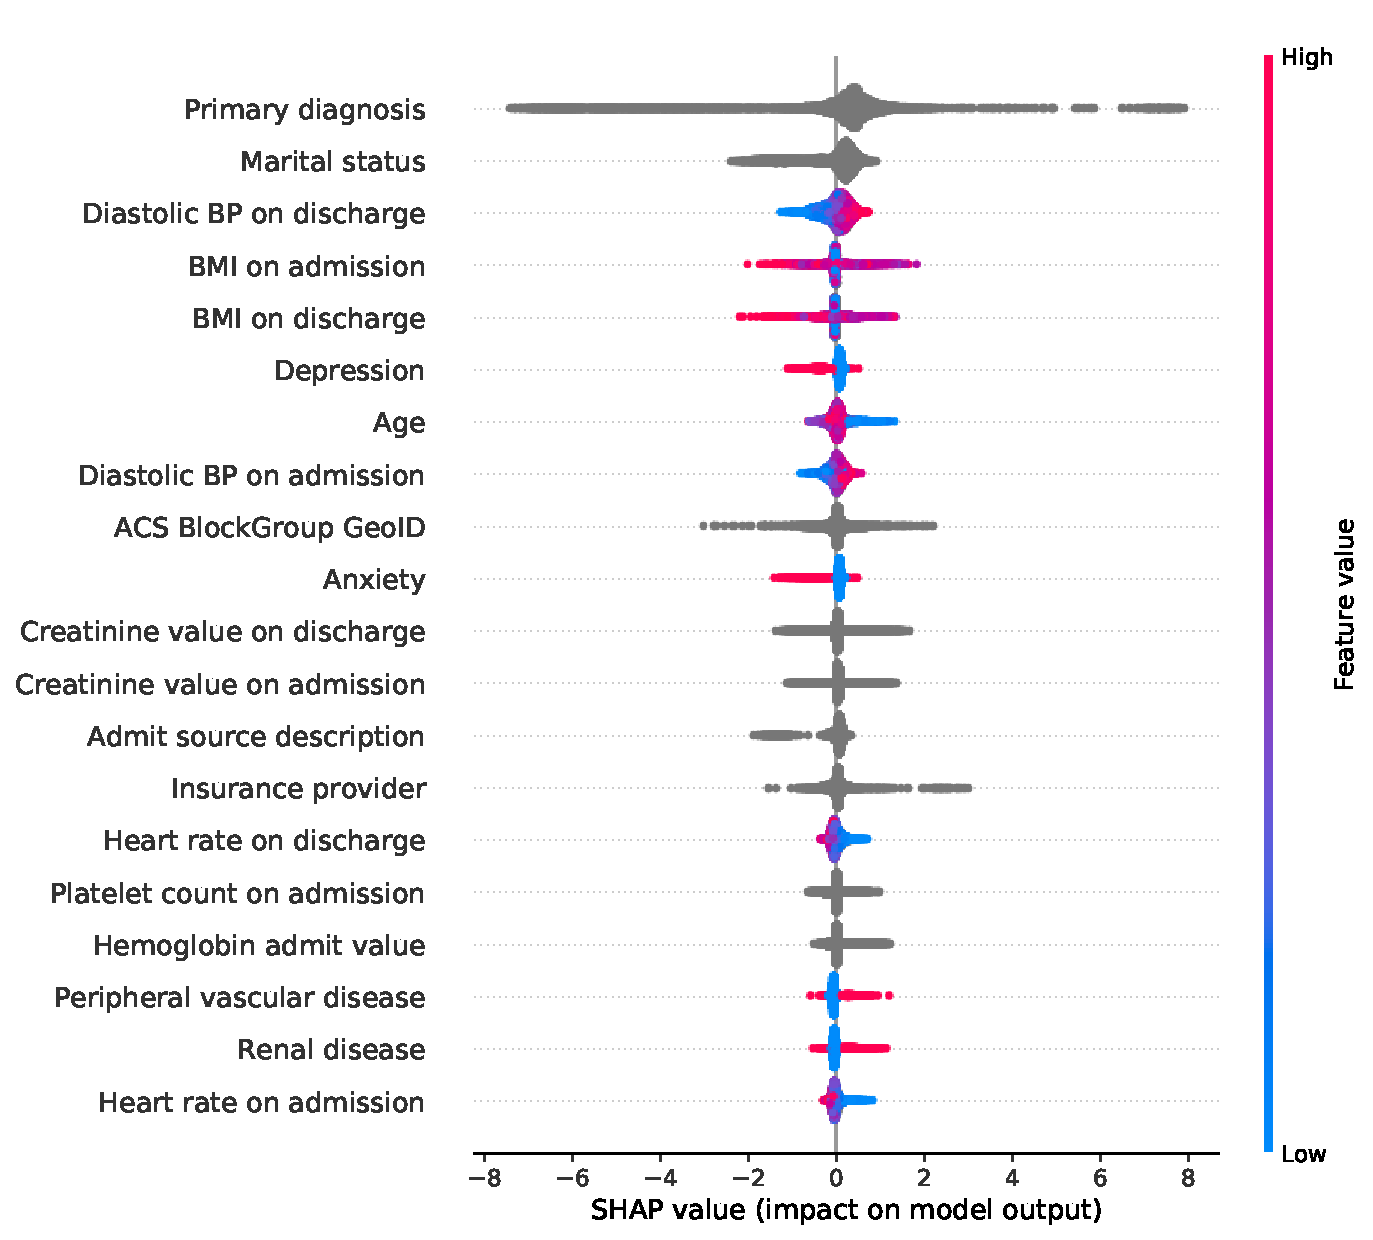
\includegraphics[height=3in,width=3in]{other/gender_SHAP_summary.pdf}
\end{subfigure}%
\hspace{5mm}%
\begin{subfigure}[t]{.45\linewidth}
    \centering
    \captionsetup[subfigure]{}
    \caption{Age.}\label{fig:shapsumage}
    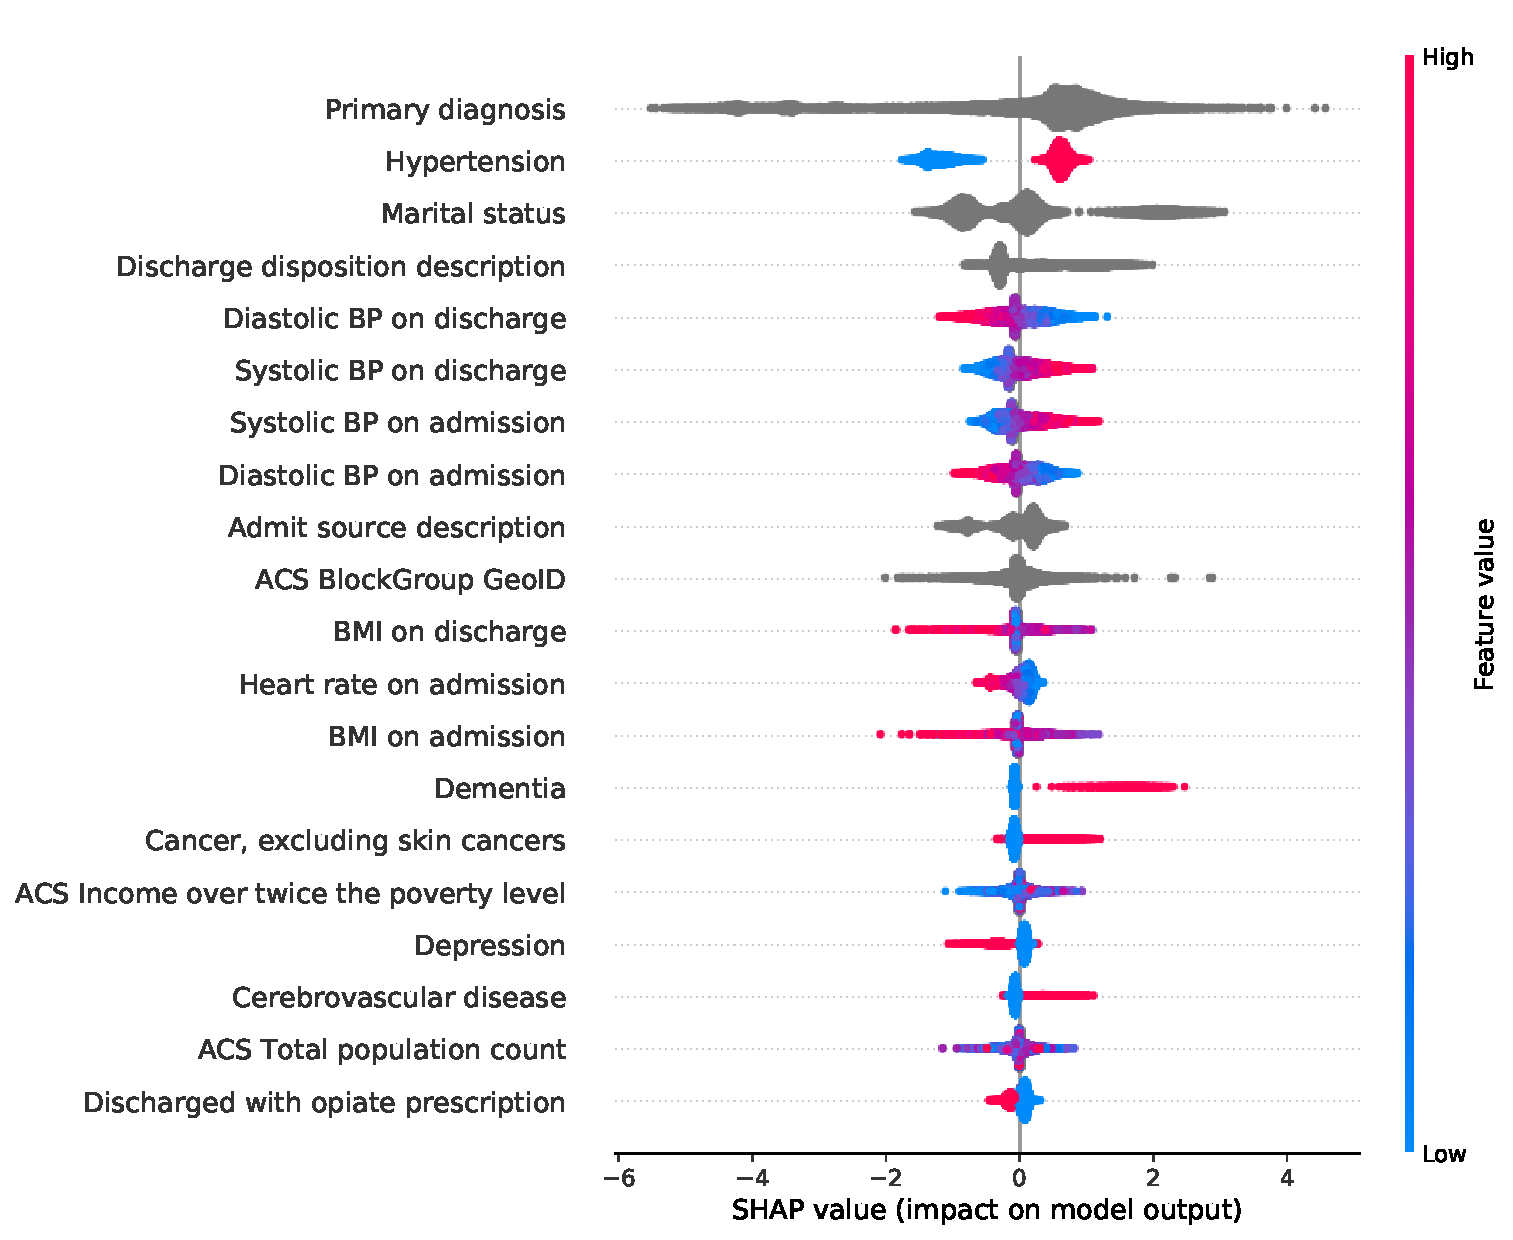
\includegraphics[height=3in,width=3in]{other/age_SHAP_summary.pdf}
    % 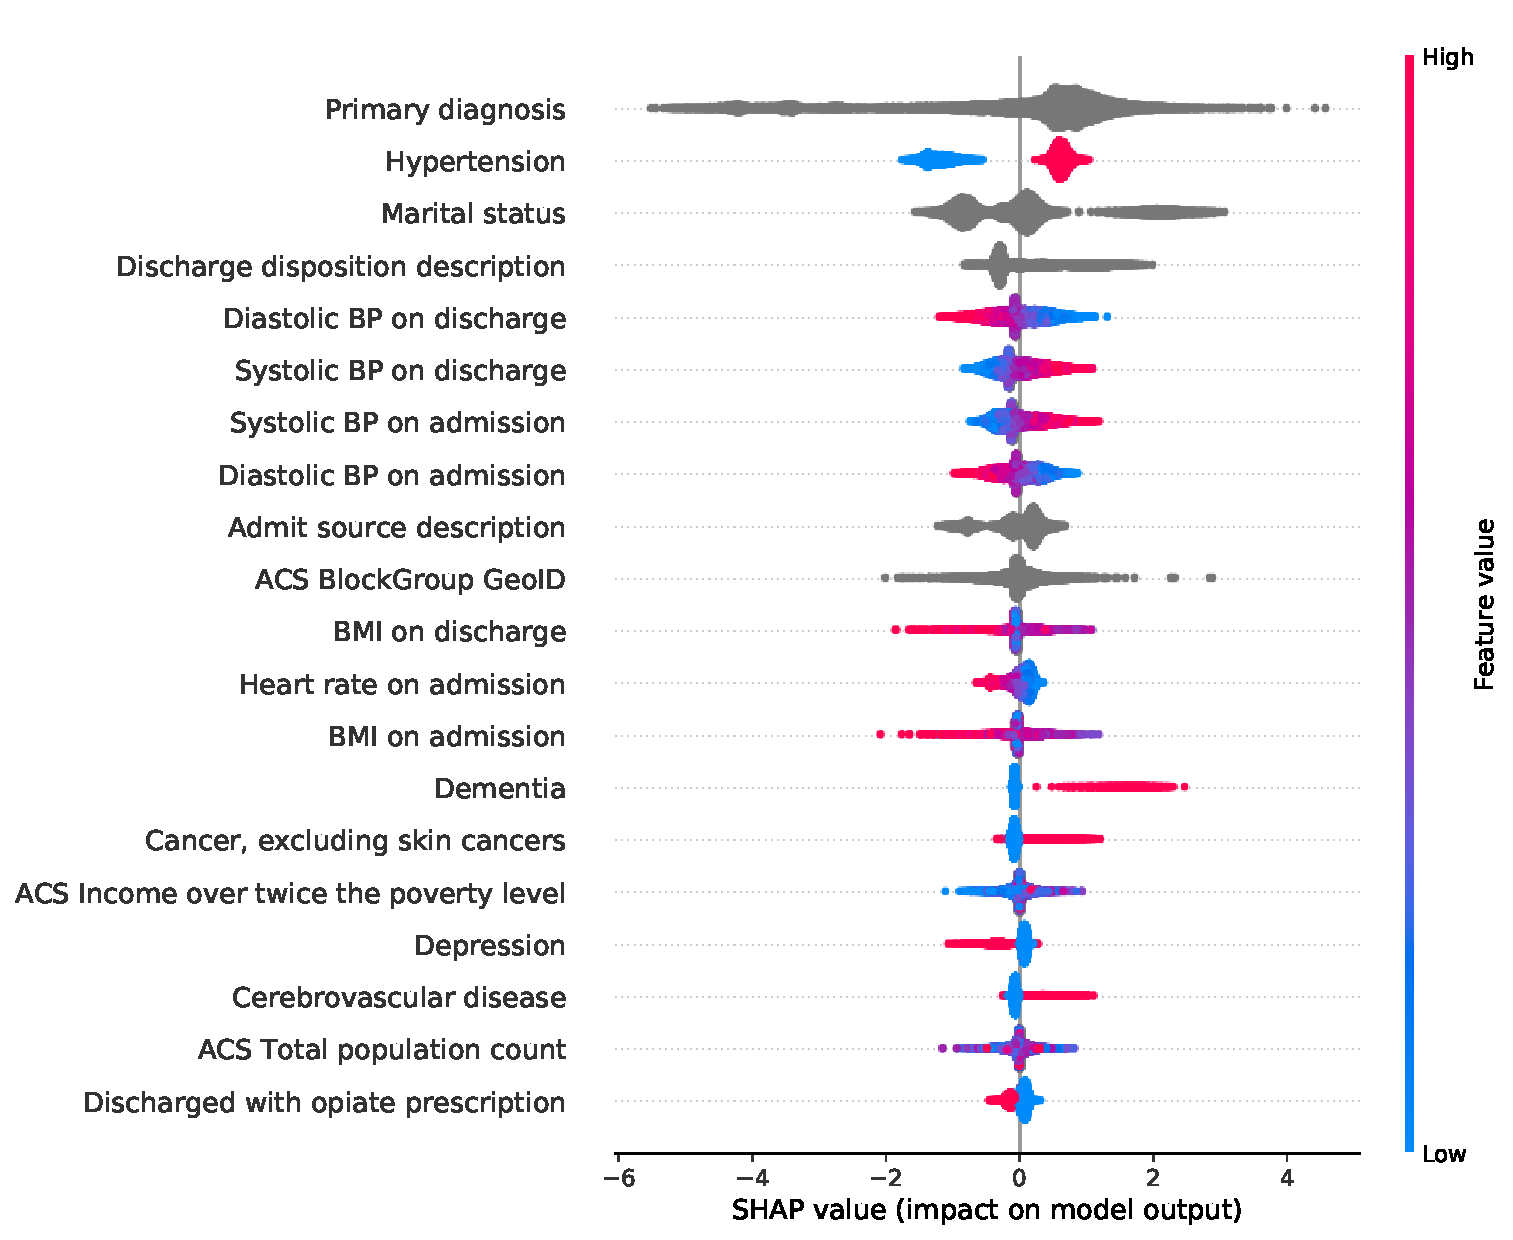
\includegraphics[width=\linewidth,keepaspectratio]{other/age_SHAP_summary.pdf}
\end{subfigure}%

\vspace{5mm}
% \hspace{5mm}%
\begin{subfigure}[t]{.45\linewidth}
    \centering
    \captionsetup[subfigure]{}
    \caption{Race. }\label{fig:shapsumrace}
    % \vspace{5mm}
    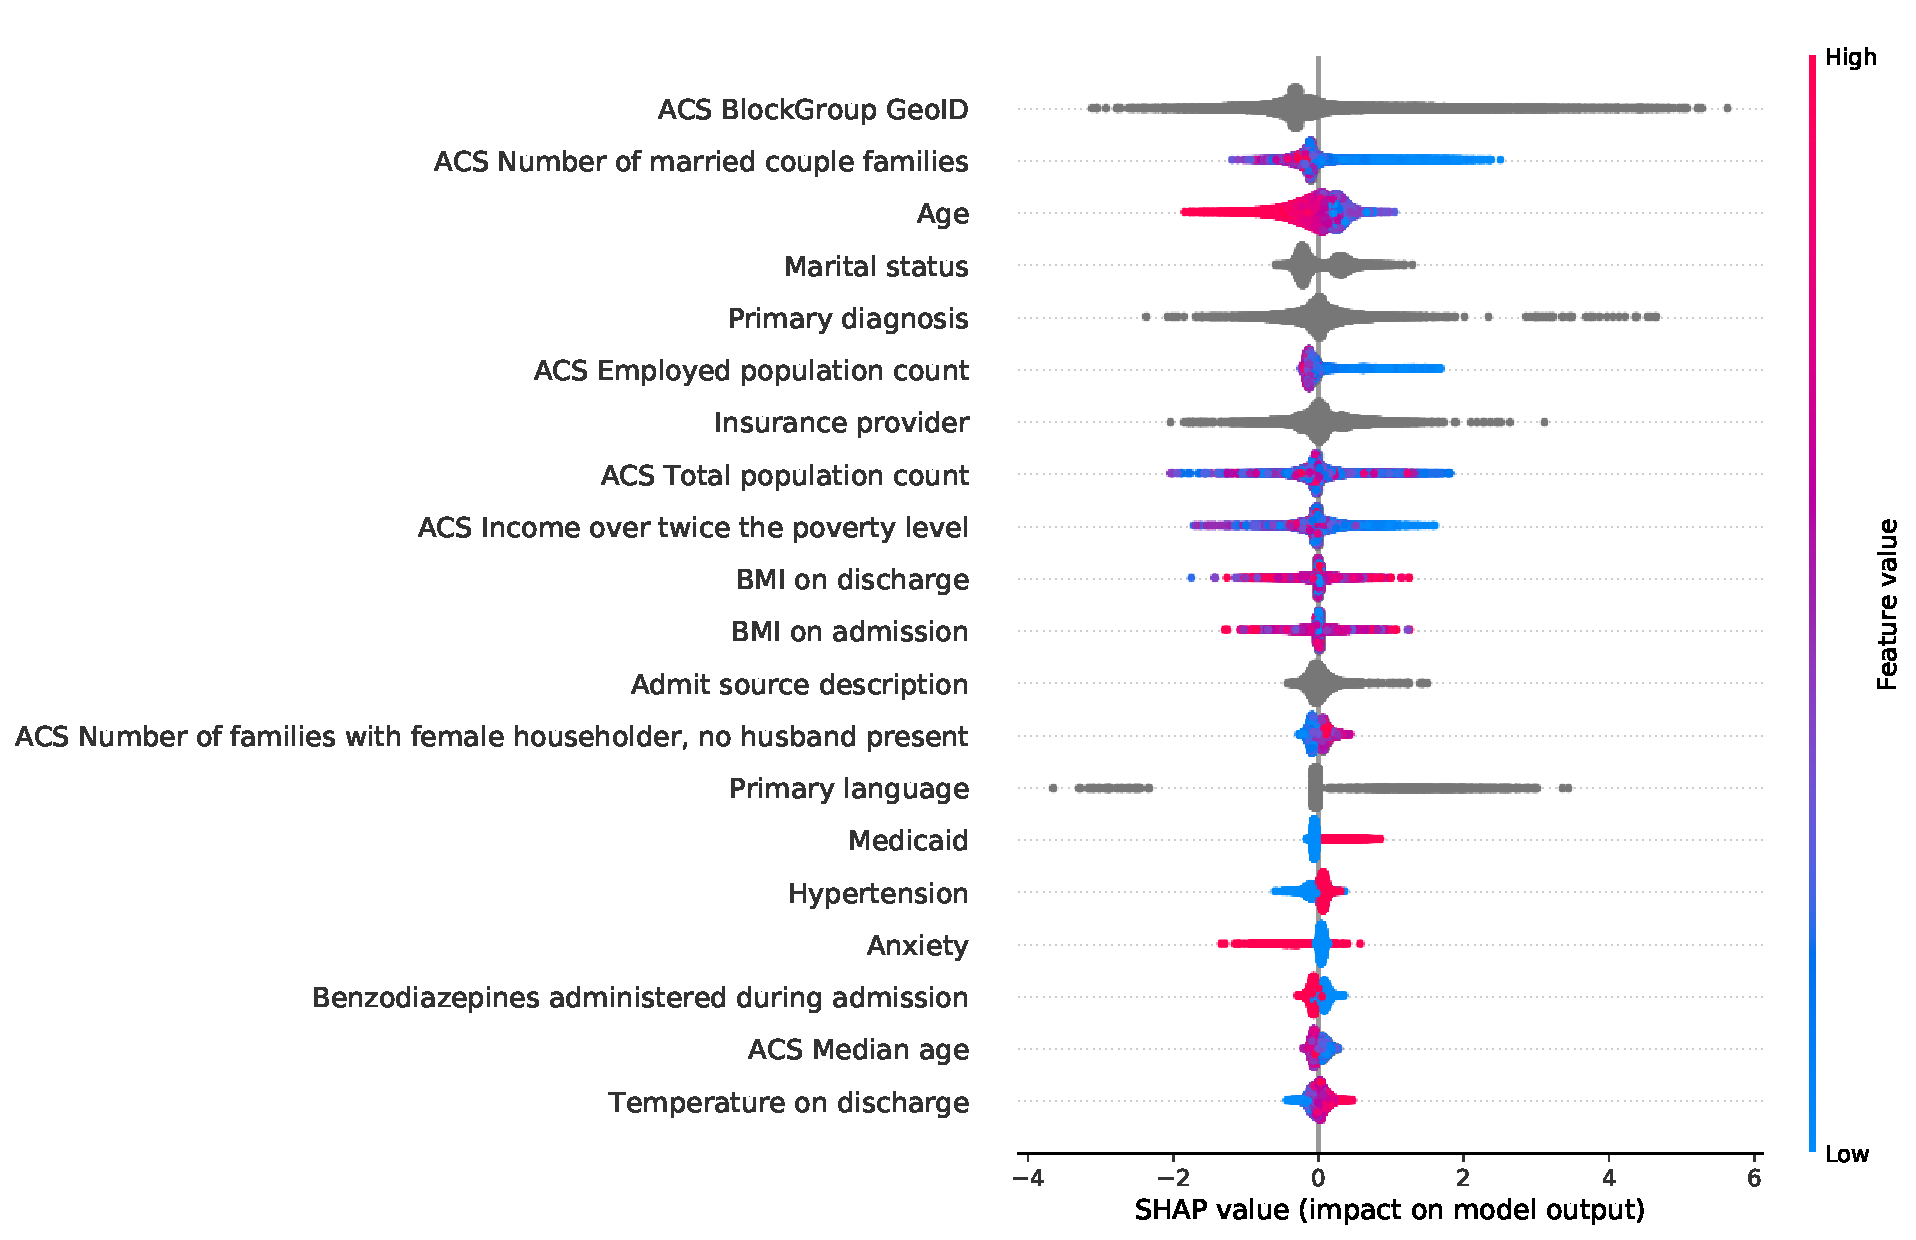
\includegraphics[height=2.7in,width=3in]{other/race_SHAP_summary.pdf}
    % \def\svgwidth{width=3in} %C:\Users\hiltonc\Desktop\readmit\reports\text\figdir\other\race_SHAP_summary_test.pdf_tex
    % \subimport{/other/}{race_SHAP_summary_test.pdf_tex}
    % \input{race_SHAP_summary_test.pdf_tex}
    % 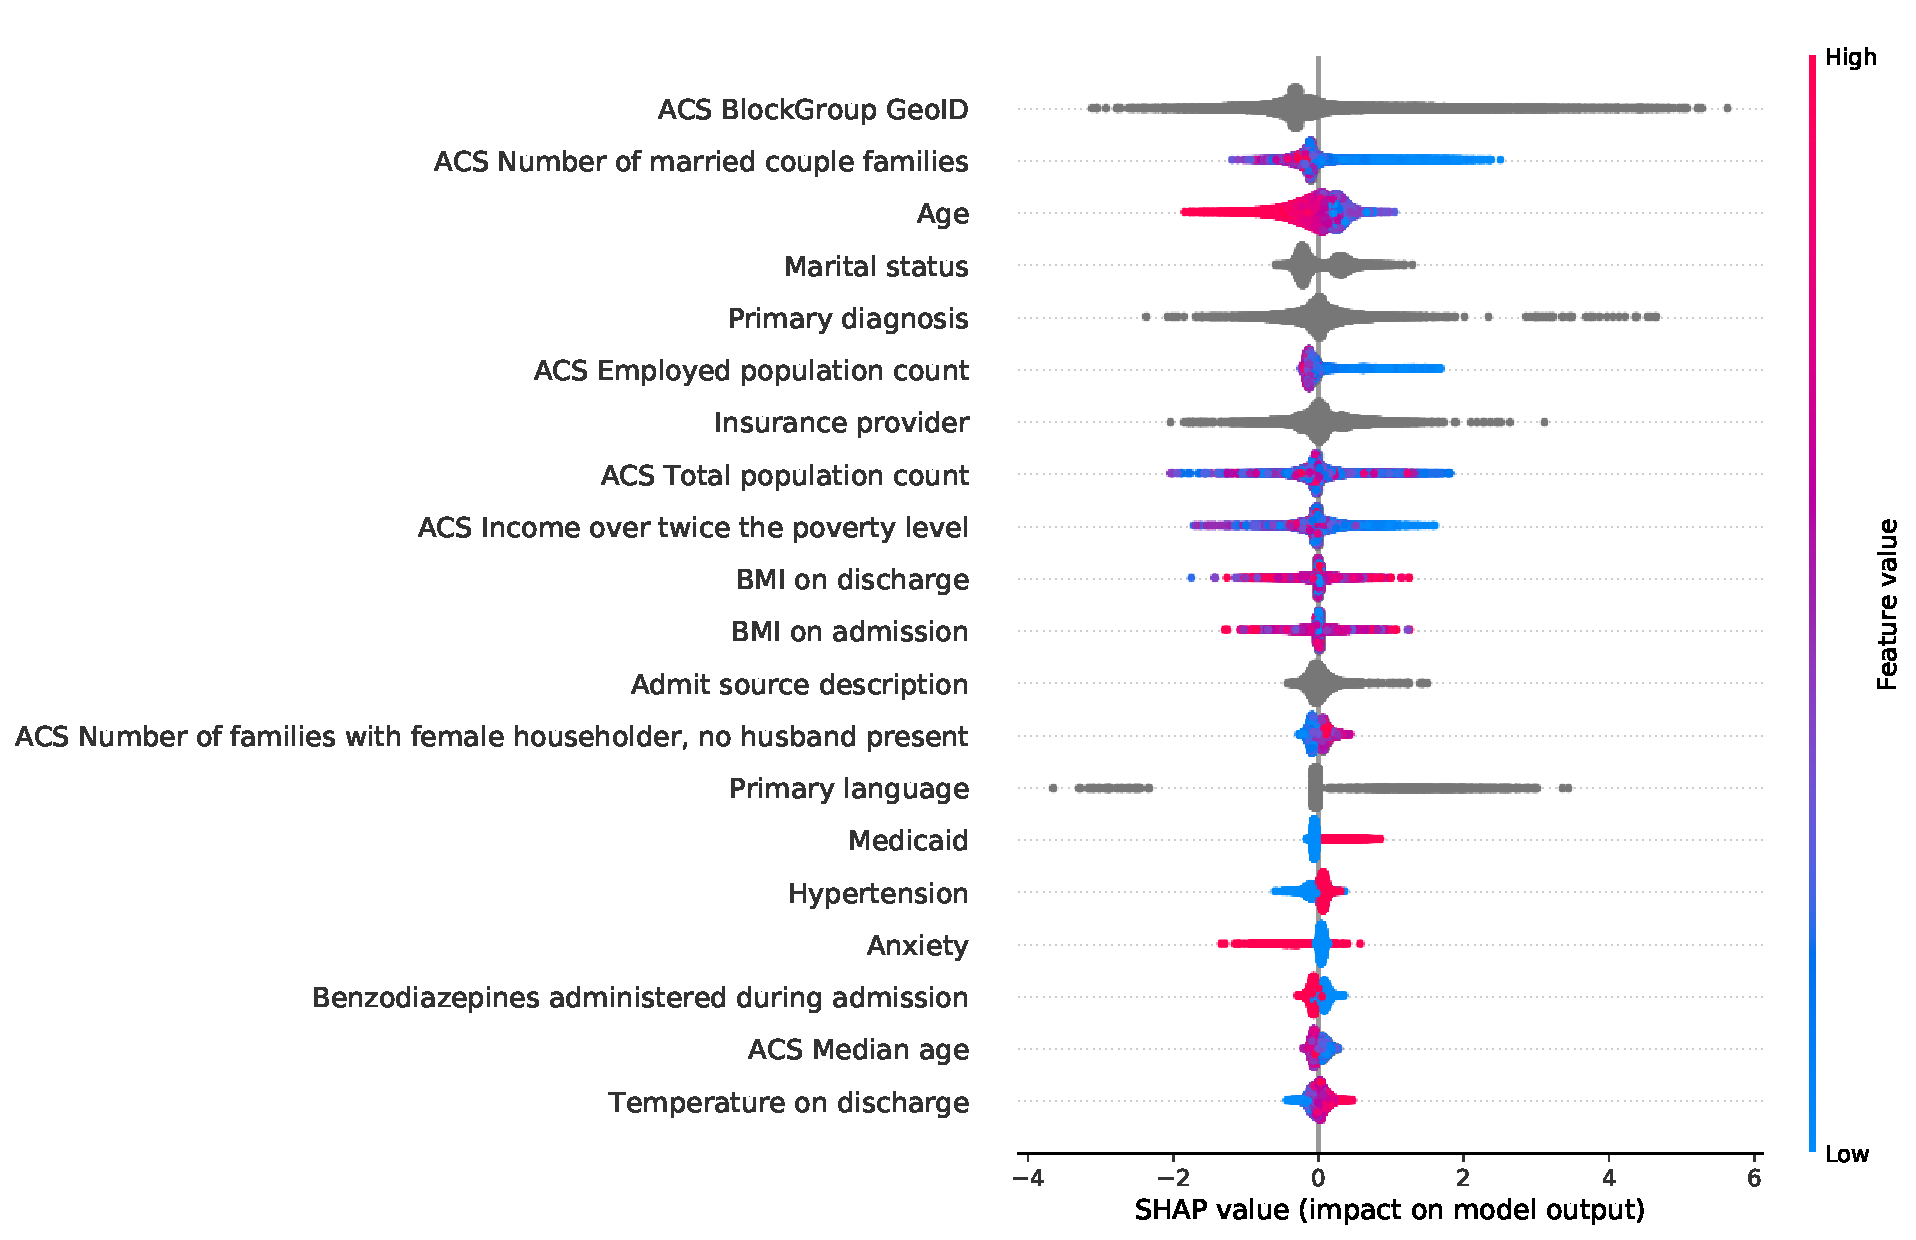
\includegraphics[width=\linewidth,keepaspectratio]{other/race_SHAP_summary.pdf}
\end{subfigure}%
\hspace{5mm}%
\begin{subfigure}[t]{.45\linewidth}
    \centering
    \captionsetup[subfigure]{}
    \caption{Financial class.}\label{fig:shapsuminsurance}
    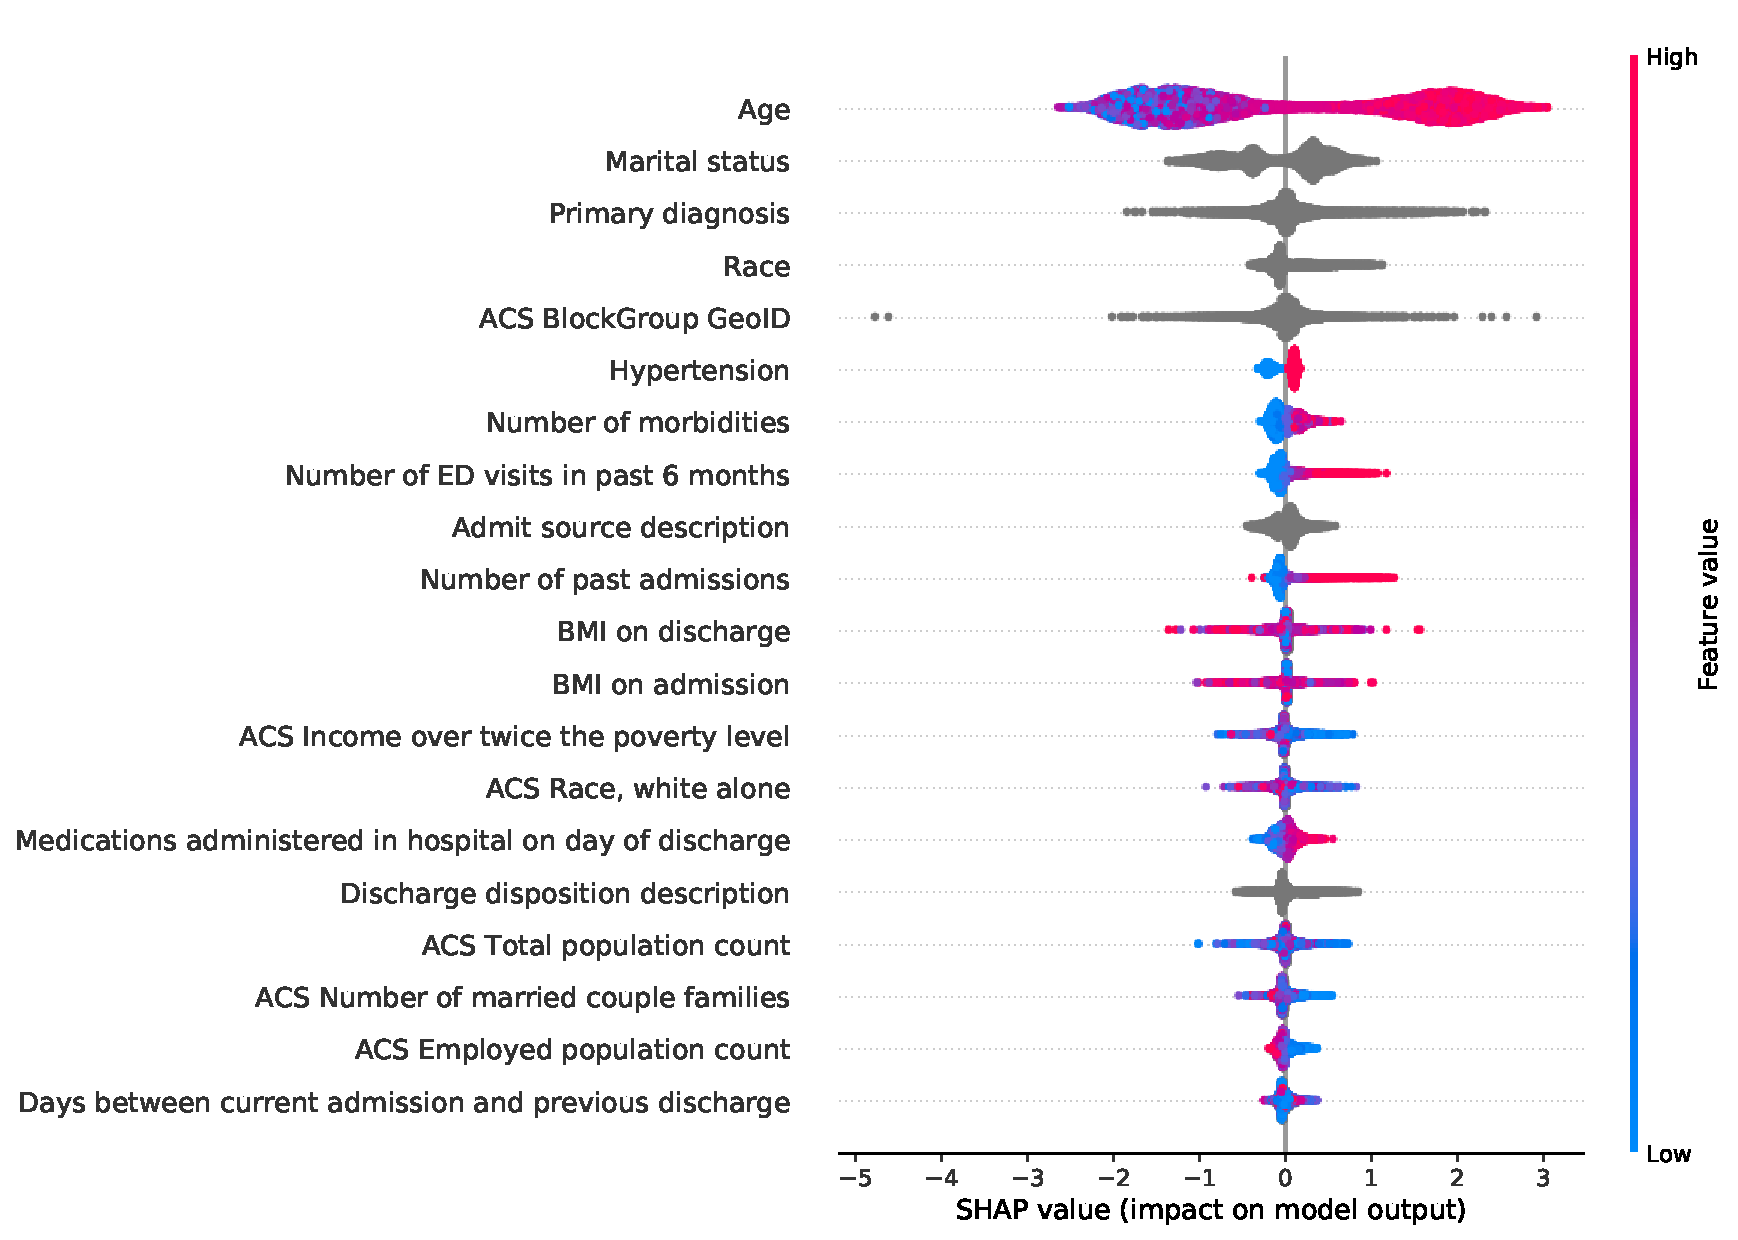
\includegraphics[height=2.7in,width=3in]{other/insurance_SHAP_summary.pdf}
    % 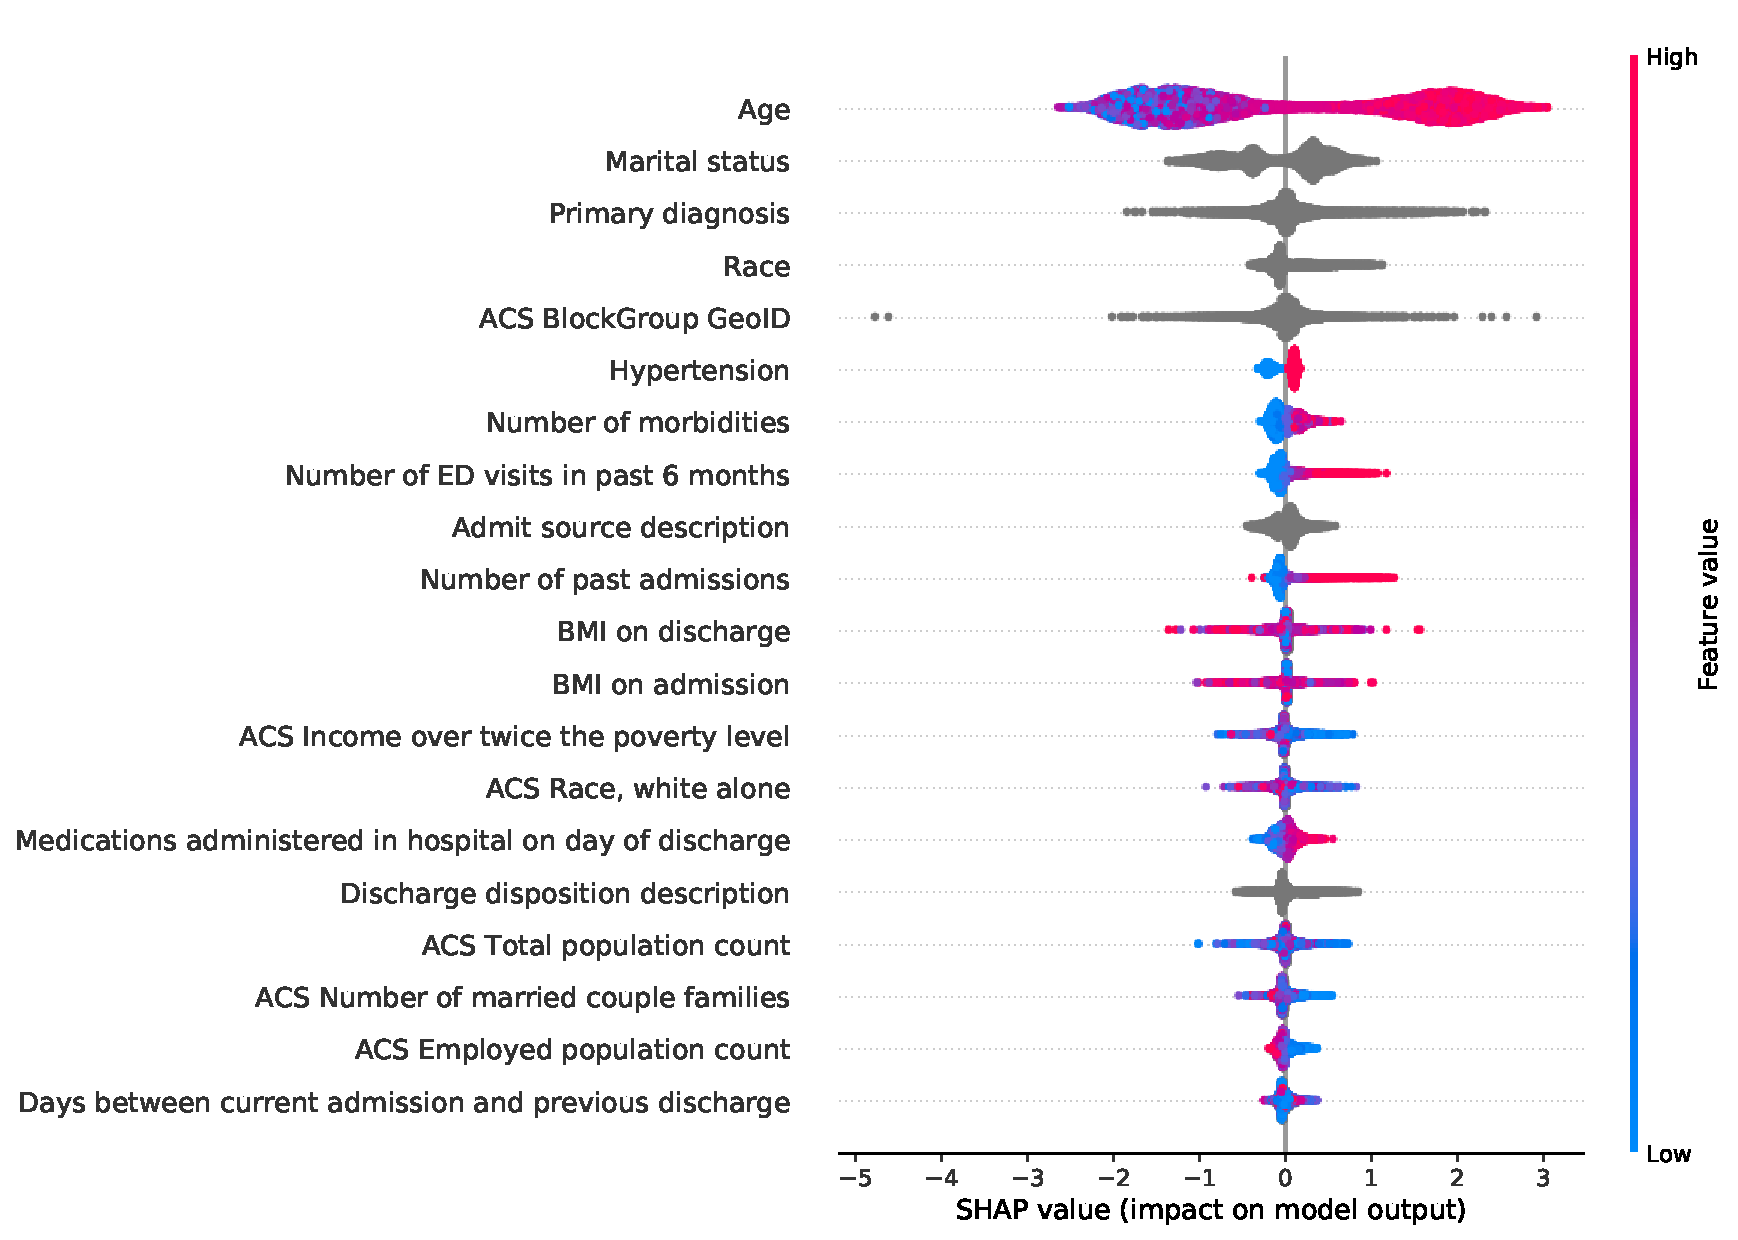
\includegraphics[width=\linewidth,keepaspectratio]{other/insurance_SHAP_summary.pdf}
\end{subfigure}%

% \noindent
% \rule[1ex]{width=\linewidth}{0.5pt}
\caption{\textbf{Prediction of Patient Characteristics.} \\
Panels~\ref{fig:shapsumgender},~\ref{fig:shapsumage},~\ref{fig:shapsumrace}, and~\ref{fig:shapsuminsurance} 
show the most impactful features on prediction, 
along with the impact of high or low values for numeric features.
}\label{fig:otherfig}
\end{adjustbox}
\end{figure}
\clearpage
\pagestyle{fancy}%
% \noindent
% \rule[1ex]{width=\linewidth}{0.5pt}
% in{minipage}[t][0.5\textheight][t]{\textwidth} 





% \pagestyle{fancy}
% \onecolumn{}
% \begin{figure}
% \begin{adjustbox}{minipage=1.0\linewidth,frame}
% \vspace{2.5mm}
% \centering

% \begin{subfigure}[t]{.3\linewidth}
% % \centering
% \captionsetup[subfigure]{}
% \caption[t]{Receiver operator characteristic curve for gender.}\label{fig:rocgender}
% 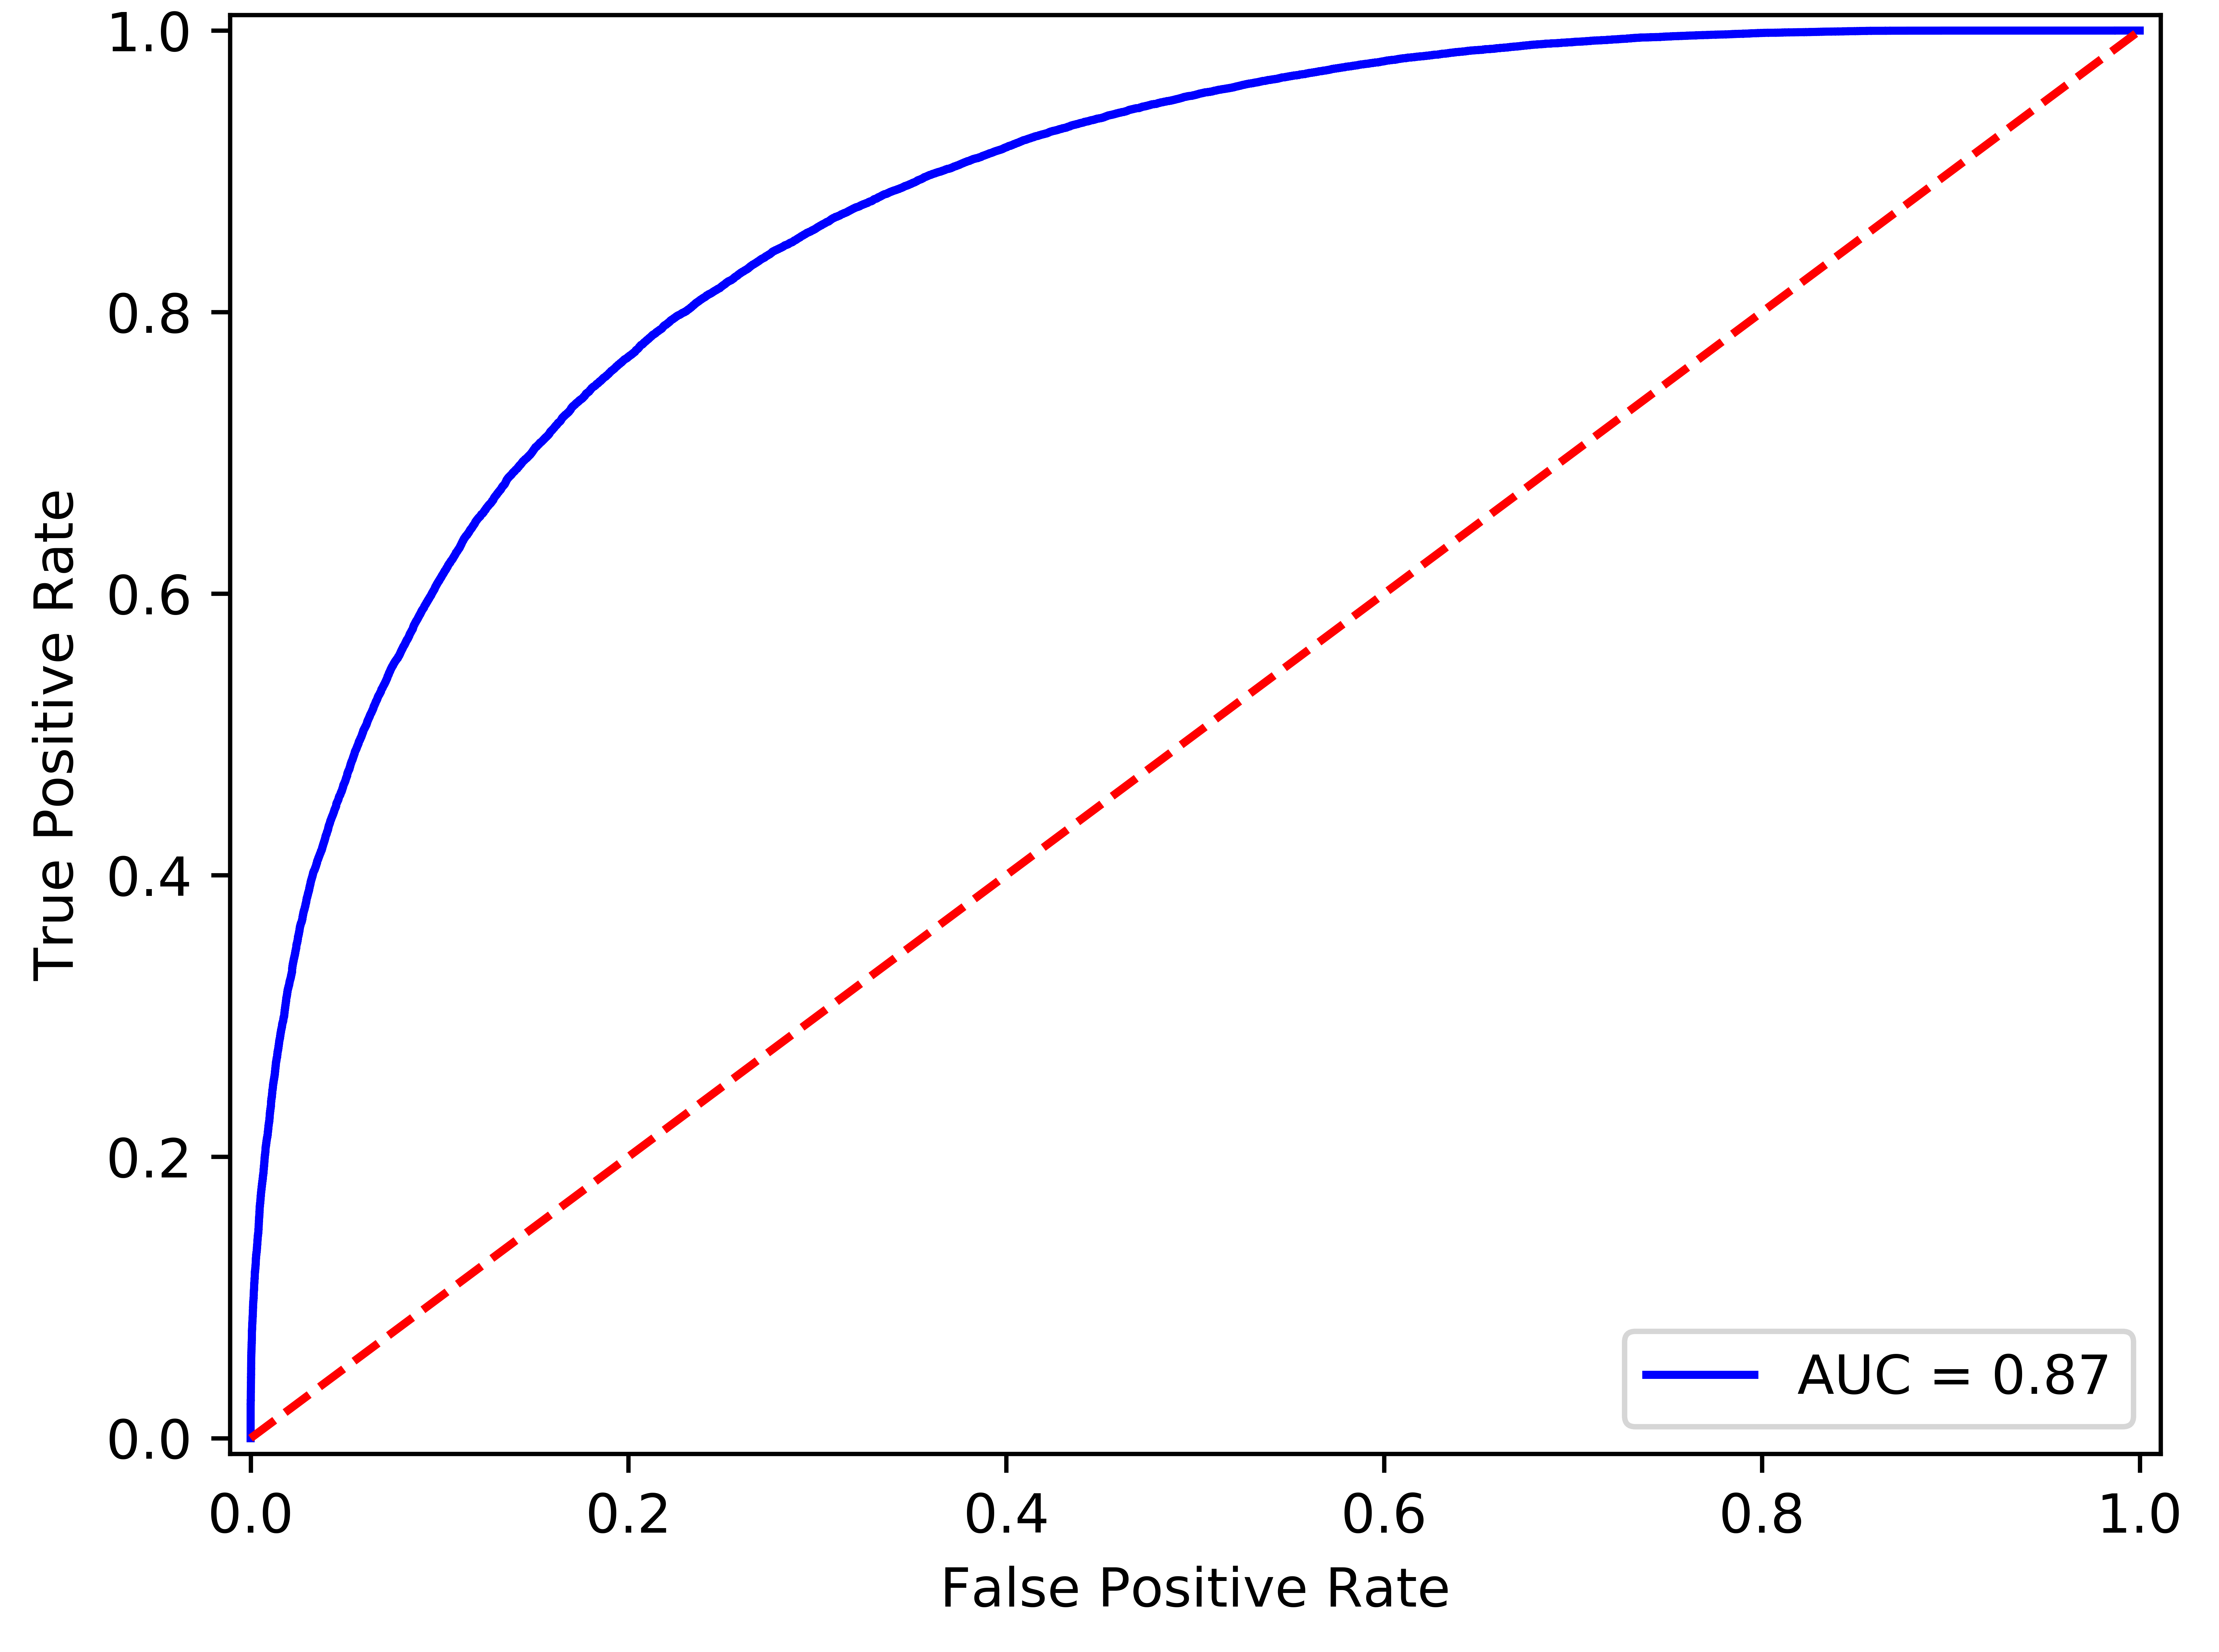
\includegraphics[width=\linewidth,height=.2\textheight,keepaspectratio]{other/gender_ROC.png}
% \end{subfigure}%
% \hspace{5mm}%
% \begin{subfigure}[t]{.5\linewidth}
%     \centering
%     \captionsetup[subfigure]{}
%     \caption{Summary of most impactful features for gender.}\label{fig:shapsumgender}
%     \includegraphics[width=\linewidth,keepaspectratio]{other/gender_SHAP_summary.png}
% \end{subfigure}%

% \begin{subfigure}[t]{.3\linewidth}
%     \centering
%     \captionsetup[subfigure]{}
%     \caption[t]{Receiver operator characteristic curve for race.}\label{fig:rocrace}
%     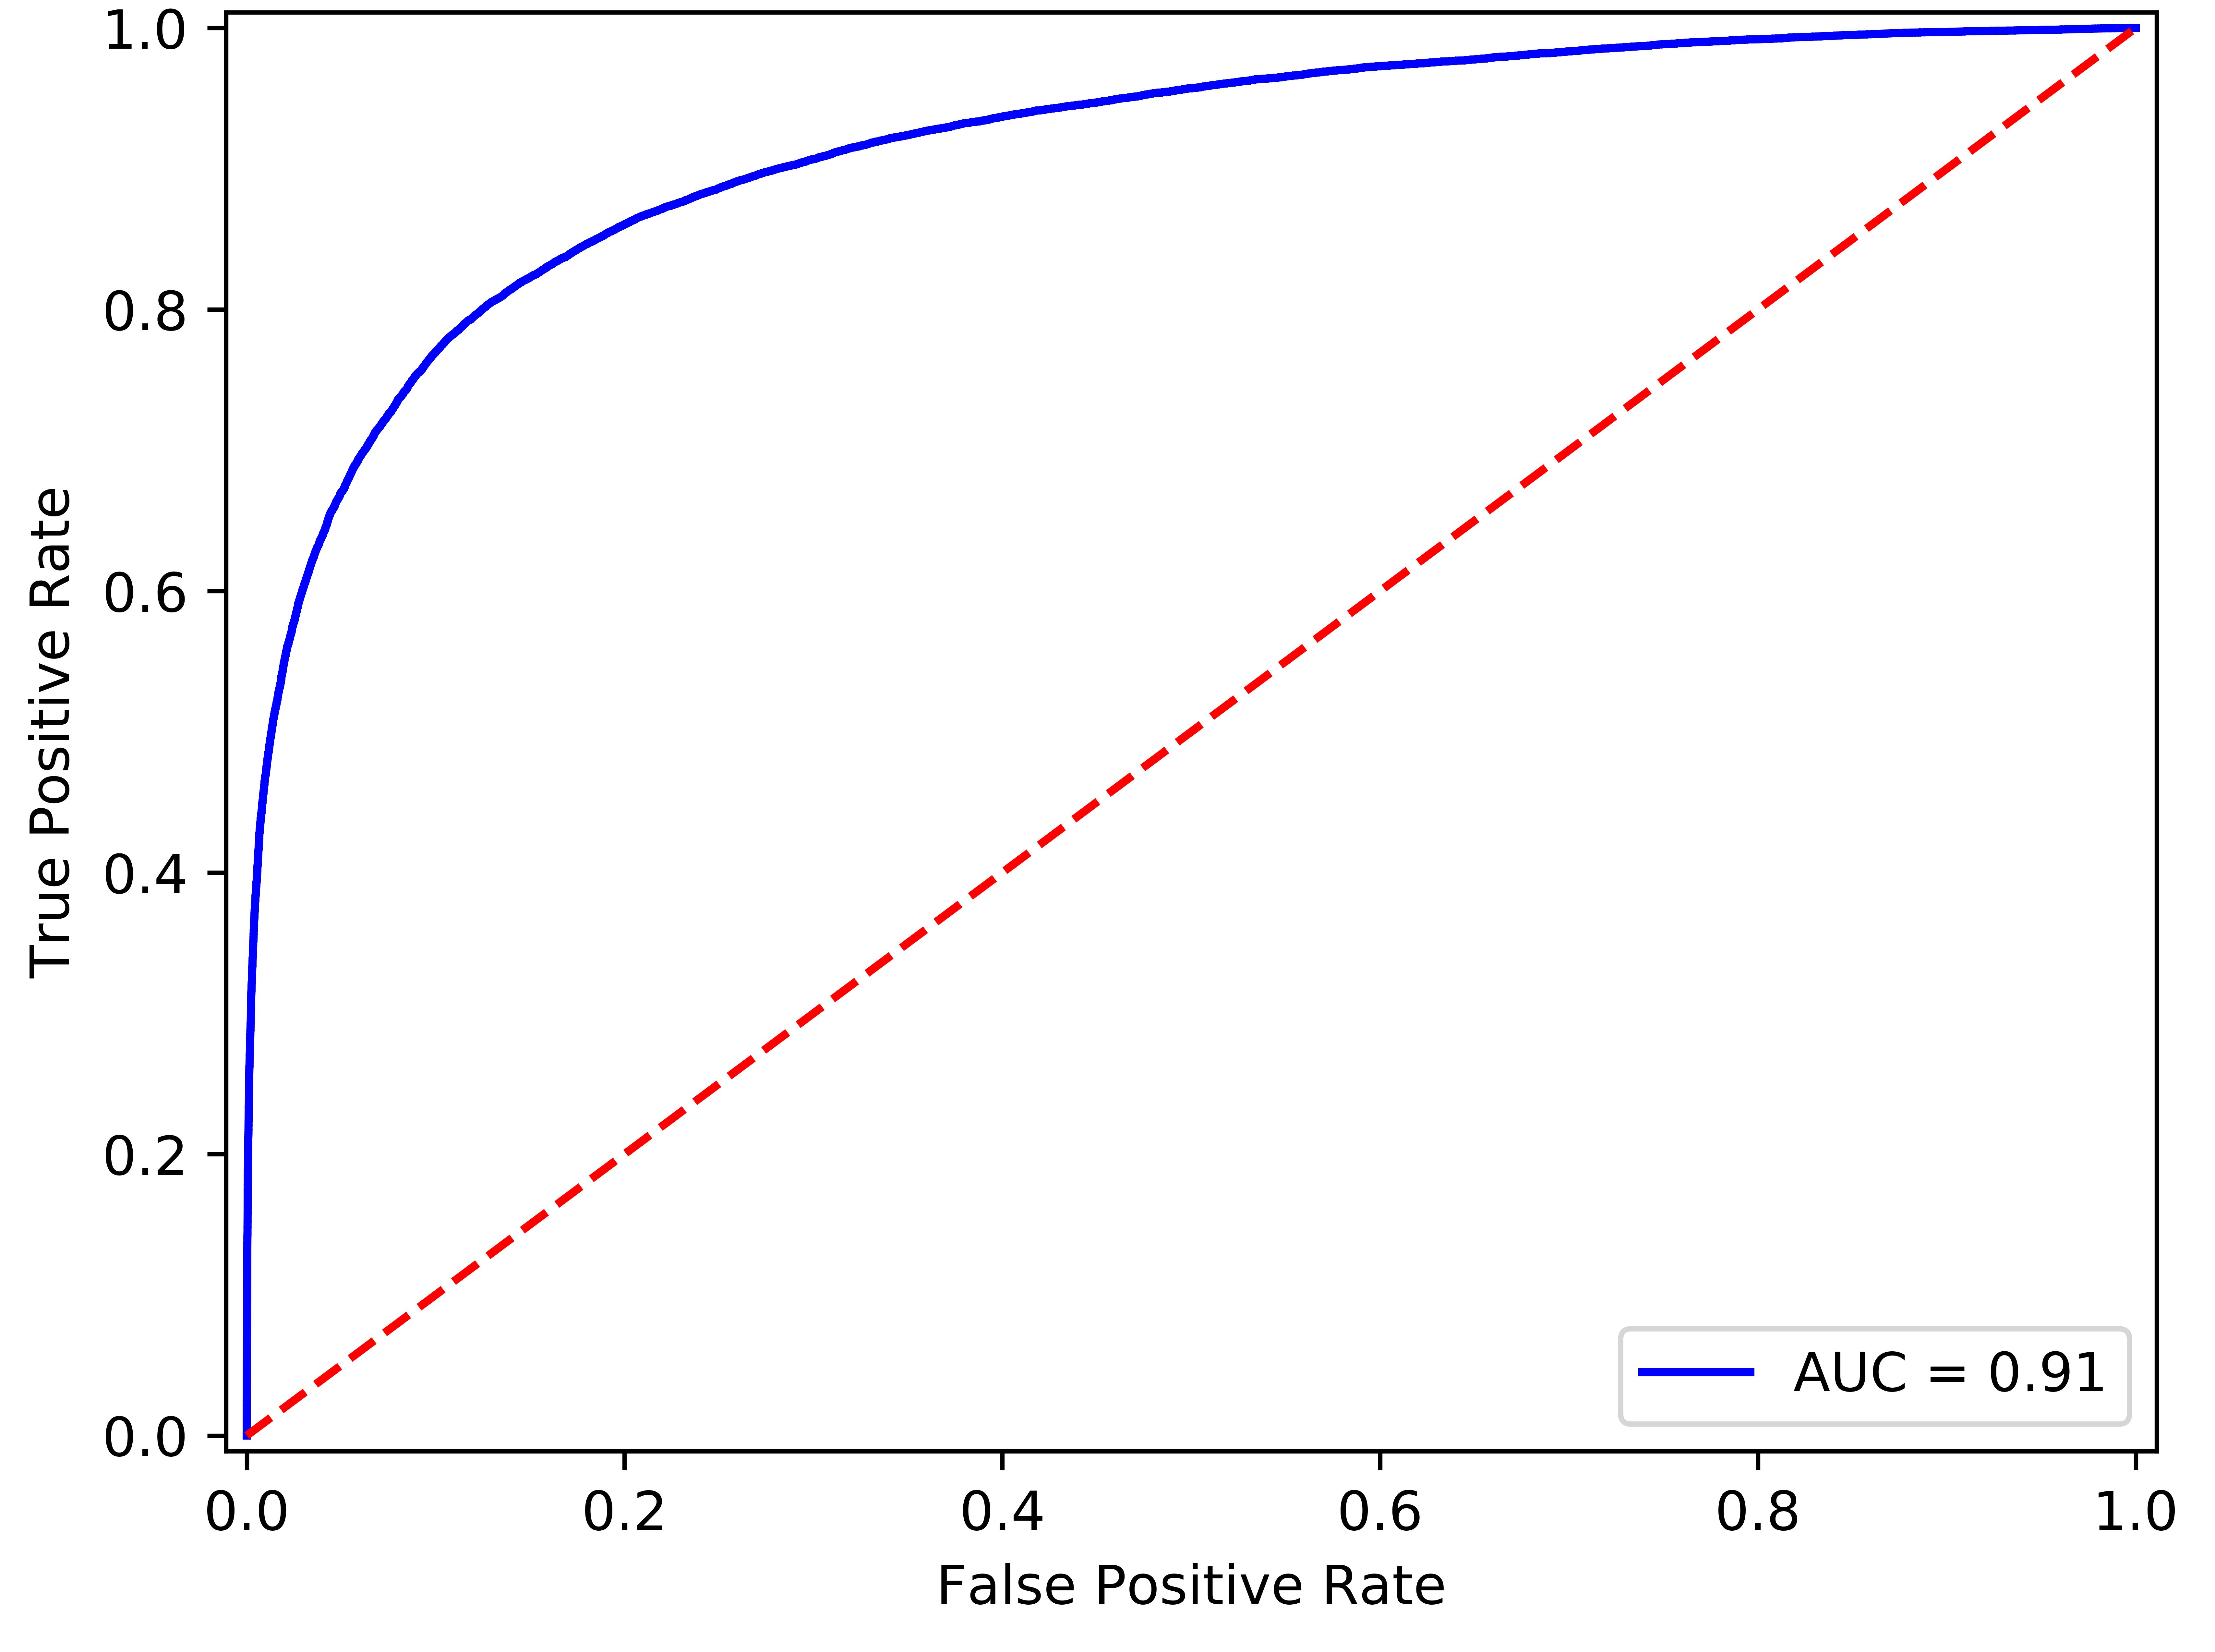
\includegraphics[width=\linewidth,height=.2\textheight,keepaspectratio]{other/race_ROC.png}
% \end{subfigure}%
% \hspace{5mm}%
% \begin{subfigure}[t]{.5\linewidth}
%     \centering
%     \captionsetup[subfigure]{}
%     \caption{Summary of most impactful features for race.}\label{fig:shapsumrace}
%     \includegraphics[width=\linewidth,keepaspectratio]{other/race_SHAP_summary.png}
% \end{subfigure}%

% \begin{subfigure}[t]{.3\linewidth}
%     \centering
%     \captionsetup[subfigure]{}
%     \caption[t]{Receiver operator characteristic curve for financial class.}\label{fig:rocinsurance}
%     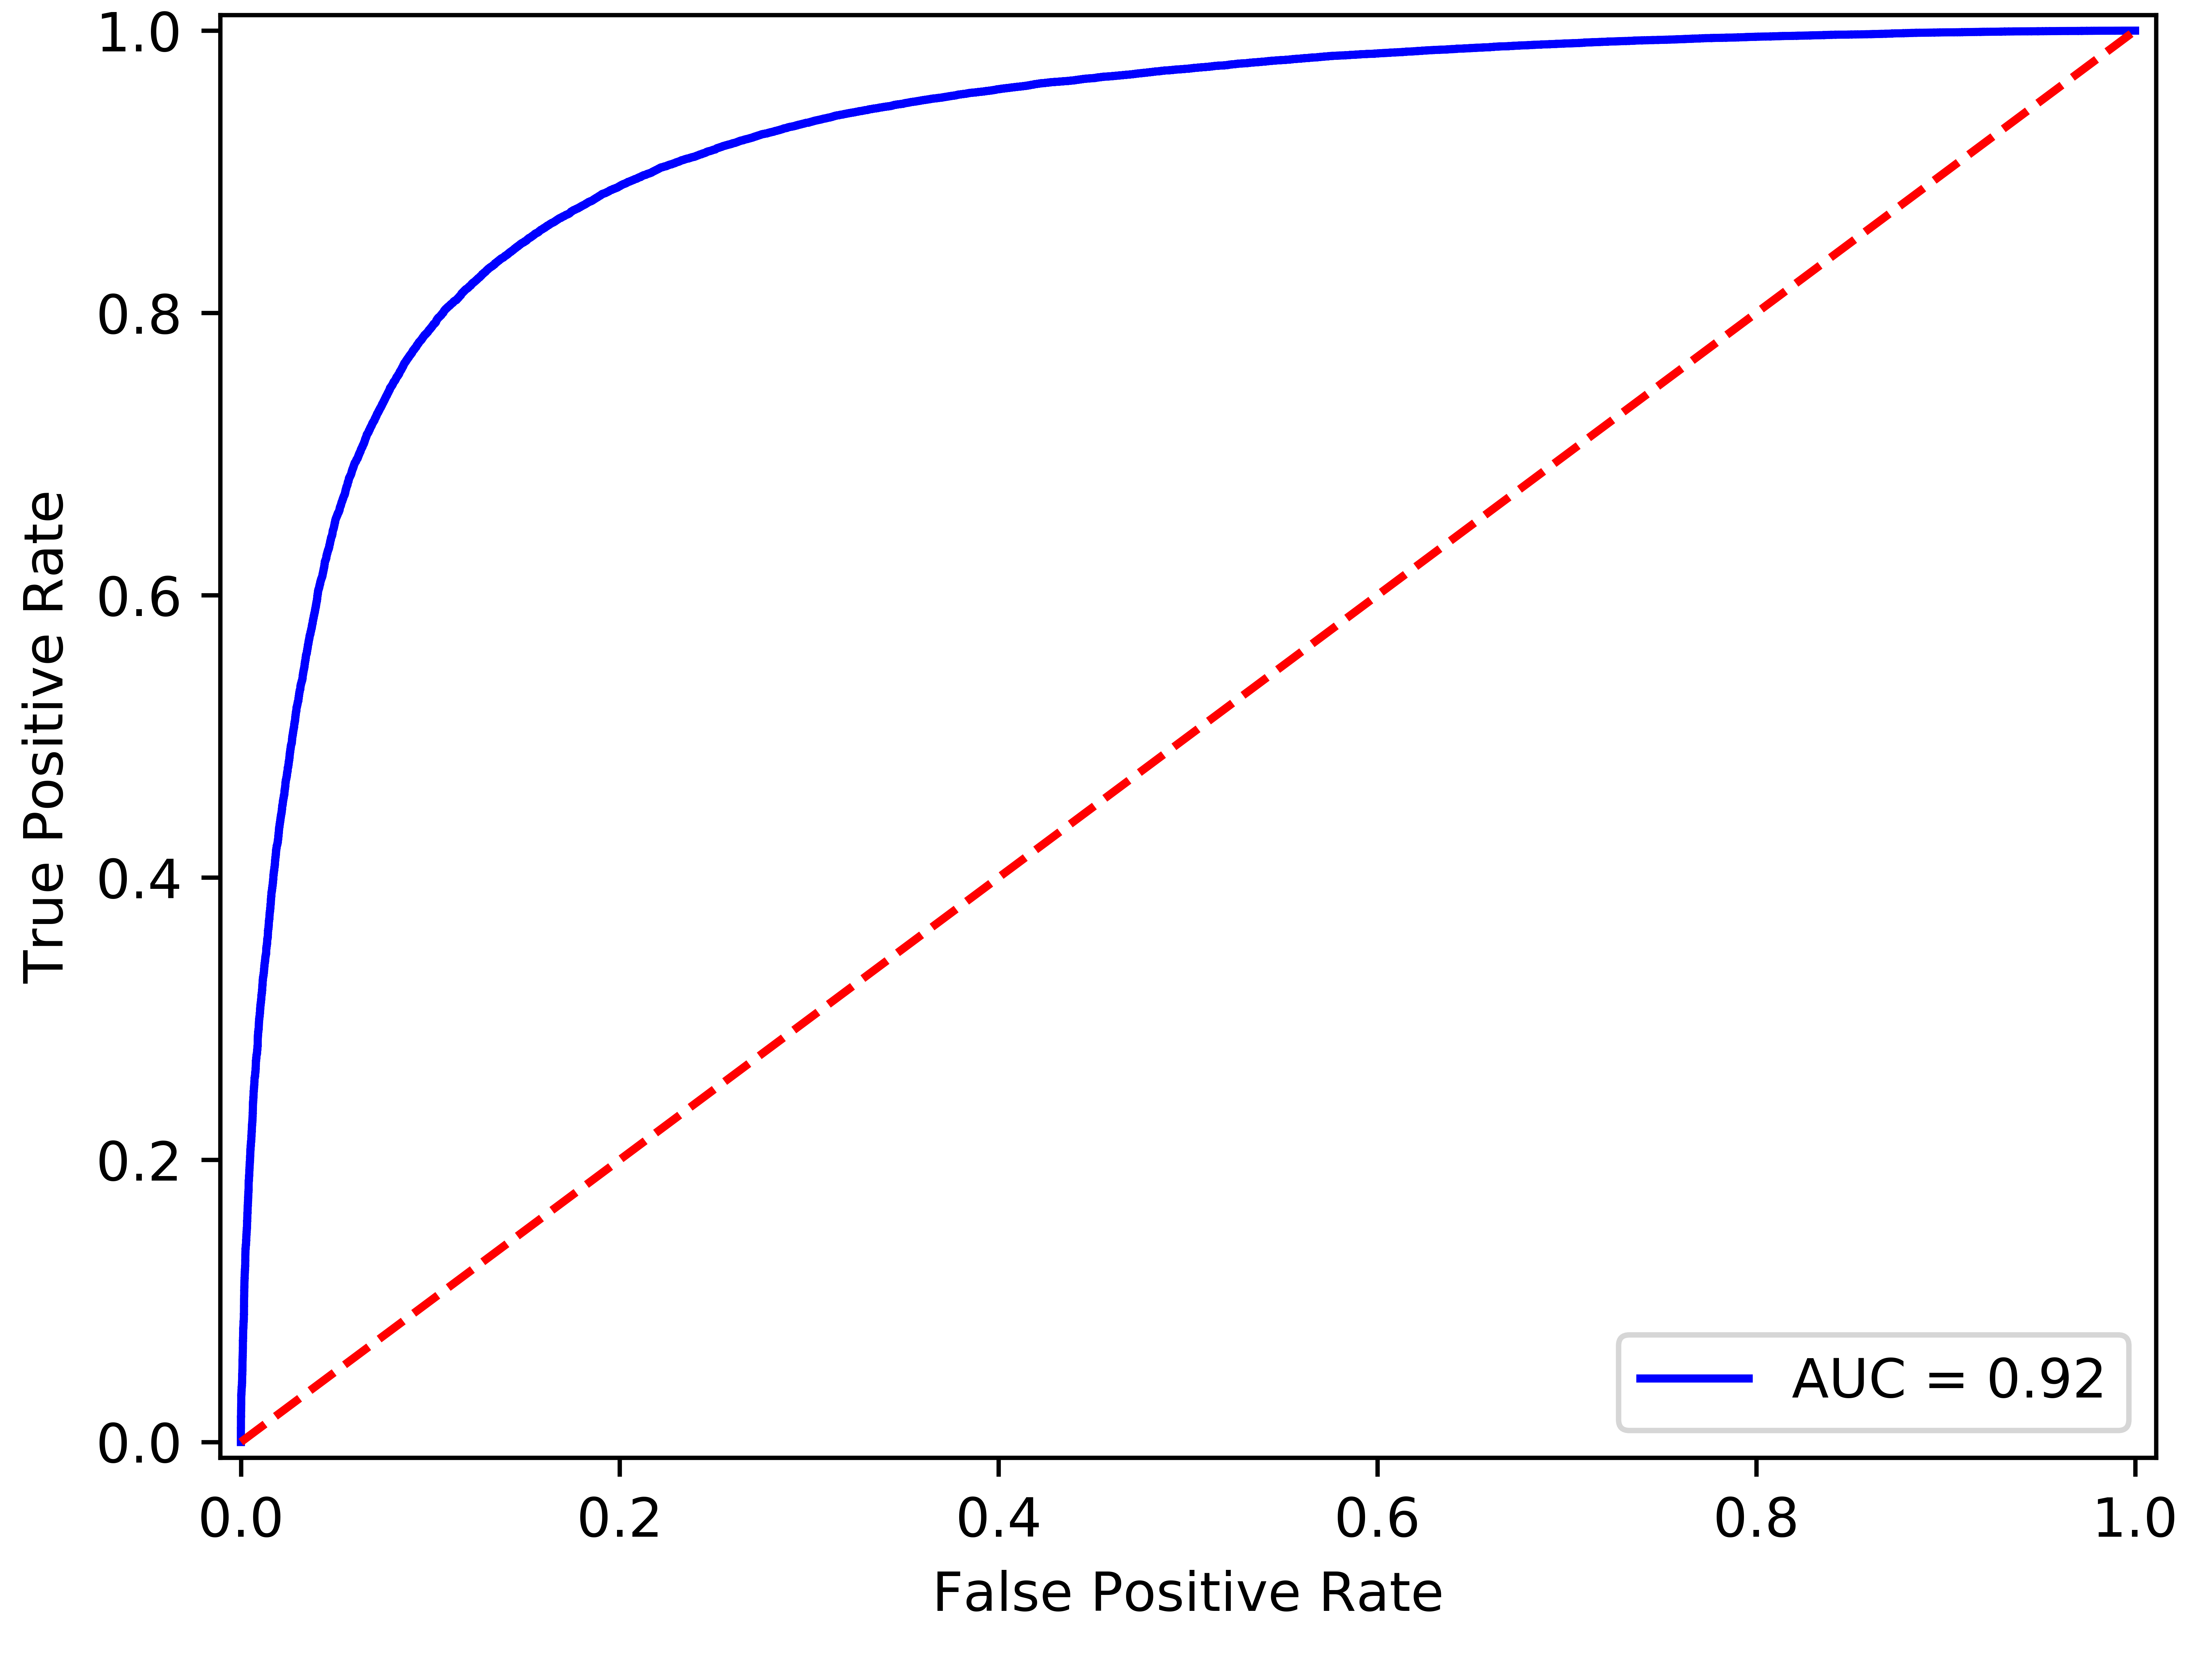
\includegraphics[width=\linewidth,height=.2\textheight,keepaspectratio]{other/insurance_ROC.png}
% \end{subfigure}%
% \hspace{5mm}%
% \begin{subfigure}[t]{.5\linewidth}
%     \centering
%     \captionsetup[subfigure]{}
%     \caption{Summary of most impactful features for financial class.}\label{fig:shapsuminsurance}
%     \includegraphics[width=\linewidth,keepaspectratio]{other/insurance_SHAP_summary.png}
% \end{subfigure}%

% % \noindent
% % \rule[1ex]{width=\linewidth}{0.5pt}
% \caption{\textbf{Prediction of Patient Characteristics.} \\
% Model performance curves are shown for binary classification (Panels \ref{fig:rocgender}, \ref{fig:rocrace}, \ref{fig:rocinsurance}).
% Panels \ref{fig:shapsumgender}, \ref{fig:shapsumrace}, \ref{fig:shapsuminsurance} 
% show the most impactful features on prediction, 
% along with the impact of high or low values for numeric features.
% }\label{fig:otherfig}
% \end{adjustbox}
% \end{figure}
% \clearpage
% \pagestyle{fancy}%
% % \noindent
% % \rule[1ex]{width=\linewidth}{0.5pt}
% % in{minipage}[t][0.5\textheight][t]{\textwidth} 